\documentclass{standalone}
\usepackage{tikz}


\begin{document}
 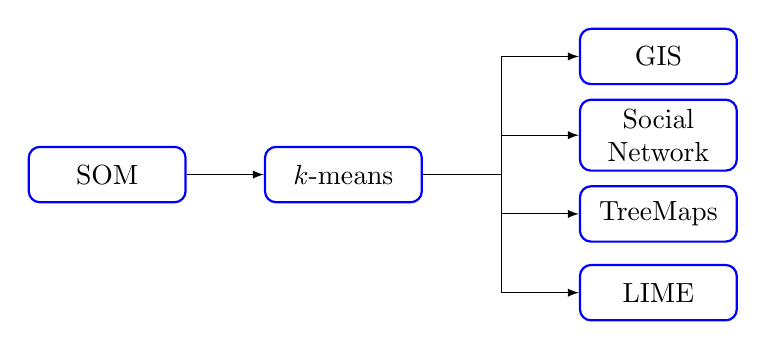
\begin{tikzpicture}[%
 auto,
 block/.style={
 	rectangle,
 	draw=blue,
 	thick,
 	fill=white,
 	text width=5em,
 	align=center,
 	rounded corners,
 	minimum height=2em
 },
 block1/.style={
 	rectangle,
 	draw=blue,
 	thick,
 	fill=blue!20,
 	text width=5em,
 	align=center,
 	rounded corners,
 	minimum height=2em
 },
 line/.style={
 	draw,thick,
 	-latex',
 	shorten >=2pt
 },
 cloud/.style={
 	draw=red,
 	thick,
 	ellipse,
 	fill=red!20,
 	minimum height=1em
 }
 ]
  \draw (-7,-3.5) node[block] (A) {SOM};
 \draw (-4,-3.5) node[block] (C) {$k$-means};
 \path (0,-3) node[block] (G) {Social Network}
 (0,-4) node[block] (H) {TreeMaps}
 (0,-5) node[block] (I) {LIME}
 (0,-2) node[block] (J) {GIS};
\draw (C.east) -- ++(0,0) coordinate (linga);
\draw (linga) -- ++(1,0) coordinate (hling);
\draw[-latex] (hling) |- (J.west);
\draw[-latex] (hling) |- (H.west);
\draw[-latex] (hling) |- (I.west);
\draw[-latex] (hling) |- (G.west);

%\draw (C.south) ++(0,-2) coordinate (LT) edge[] node[below]{Unsupervised} (LT-|C.south);
%\draw (I.south) ++(0,-0.6) coordinate (LT) edge[] node[below]{Visualization} (LT-|I.south);
\draw [-latex ,black] (A) -- (C);
 \end{tikzpicture}

\end{document}